\documentclass[12pt, a4paper]{article}

% ---- packages ----
\usepackage[utf8]{inputenc}
\usepackage[T1]{fontenc}
\usepackage{amsmath, amssymb, amsfonts}
\usepackage{graphicx}
\usepackage{subcaption}
\usepackage[margin=1in]{geometry}
\usepackage{hyperref}
\usepackage{booktabs}
\usepackage{float}
\usepackage{enumitem}
\usepackage{listings}
\usepackage{xcolor}
\usepackage{fancyhdr}
\usepackage{titlesec}
\usepackage{caption}

\hypersetup{colorlinks=true, linkcolor=blue, citecolor=blue, urlcolor=blue}
\graphicspath{{cv_project_output/}{images/}}

% ---- header / footer ----
\pagestyle{fancy}
\fancyhf{}
\rhead{Computer Vision --- Project 5}
\lhead{Optical Flow \& Structure from Motion}
\cfoot{\thepage}

% ---- code listing style ----
\lstset{
  basicstyle=\ttfamily\small,
  breaklines=true,
  frame=single,
  backgroundcolor=\color{gray!10},
  keywordstyle=\color{blue},
  commentstyle=\color{green!50!black},
}

% ---- title ----
\title{\textbf{Optical Flow Analysis, Motion Tracking,\\and Structure from Motion}\\[6pt]
\large Computer Vision --- Module 6}
\author{Anil K Tiwari}  % <-- Replace with your name
\date{\today}

\begin{document}
\maketitle
\tableofcontents
\newpage

% ======================================================================
%  PART A: OPTICAL FLOW
% ======================================================================
\section{Part A --- Optical Flow Analysis}

\subsection{Video Selection}

Two videos with at least 30 seconds of motion were selected:

\begin{table}[H]
\centering
\begin{tabular}{lcccc}
\toprule
\textbf{Video} & \textbf{FPS} & \textbf{Frames} & \textbf{Resolution} & \textbf{Duration (s)}\\
\midrule
\texttt{sample1.mp4} & 30.0 & 901 & $1920\times1080$ & 30.03\\
\texttt{sample2.mp4} & 25.0 & 1068 & $1920\times1080$ & 42.72\\
\bottomrule
\end{tabular}
\caption{Video properties.}
\label{tab:videos}
\end{table}

\begin{itemize}
  \item \textbf{sample1}: A rotating Earth globe against a dark background --- coherent, smooth motion.
  \item \textbf{sample2}: A bird on a rock near flowing water --- strong, irregular, non-rigid motion.
\end{itemize}

\subsection{Preview Frames}

Three preview frames (beginning, middle, end of the 30-second clip) were extracted from each video for reference.

\begin{figure}[H]
\centering
\begin{subfigure}{0.32\textwidth}
  \includegraphics[width=\linewidth]{sample1_preview_1.jpg}
  \caption{Start}
\end{subfigure}
\begin{subfigure}{0.32\textwidth}
  \includegraphics[width=\linewidth]{sample1_preview_2.jpg}
  \caption{Middle}
\end{subfigure}
\begin{subfigure}{0.32\textwidth}
  \includegraphics[width=\linewidth]{sample1_preview_3.jpg}
  \caption{End}
\end{subfigure}
\caption{Preview frames from \texttt{sample1} (rotating Earth).}
\label{fig:preview1}
\end{figure}

\begin{figure}[H]
\centering
\begin{subfigure}{0.32\textwidth}
  \includegraphics[width=\linewidth]{sample2_preview_1.jpg}
  \caption{Start}
\end{subfigure}
\begin{subfigure}{0.32\textwidth}
  \includegraphics[width=\linewidth]{sample2_preview_2.jpg}
  \caption{Middle}
\end{subfigure}
\begin{subfigure}{0.32\textwidth}
  \includegraphics[width=\linewidth]{sample2_preview_3.jpg}
  \caption{End}
\end{subfigure}
\caption{Preview frames from \texttt{sample2} (bird and water).}
\label{fig:preview2}
\end{figure}


% ------------------------------------------------------------------
\subsection{Optical Flow Computation}

Dense optical flow was computed using the \textbf{Farneb\"{a}ck} method, which estimates a displacement field $(u,v)$ for every pixel between consecutive frames.

\subsubsection{Method}

Given two consecutive grayscale frames $I_{t}$ and $I_{t+1}$, the Farneb\"{a}ck algorithm approximates each neighbourhood by a quadratic polynomial and estimates the displacement that best aligns the two polynomials. The output is a dense flow field:
\[
  \mathbf{f}(x,y) = \bigl(u(x,y),\; v(x,y)\bigr),
\]
where $u$ and $v$ are the horizontal and vertical displacements, respectively.

Parameters used: \texttt{pyr\_scale=0.5, levels=3, winsize=15, iterations=3, poly\_n=5, poly\_sigma=1.2}.

\subsubsection{Visualization}

Two complementary visualizations were produced for each frame pair:

\begin{enumerate}
  \item \textbf{HSV colour-coded flow map} --- hue encodes motion direction, intensity encodes magnitude.
  \item \textbf{Sparse arrow overlay} --- arrows sampled on a grid show displacement direction and relative magnitude.
\end{enumerate}

\begin{figure}[H]
\centering
\includegraphics[width=0.95\textwidth]{sample1_evidence_frame_300.jpg}
\caption{Optical flow evidence frame from \texttt{sample1} (frame 300). Left: original. Centre: dense flow (HSV). Right: sparse arrows.}
\label{fig:flow_ev1}
\end{figure}

\begin{figure}[H]
\centering
\includegraphics[width=0.95\textwidth]{sample2_evidence_frame_250.jpg}
\caption{Optical flow evidence frame from \texttt{sample2} (frame 250). Left: original. Centre: dense flow (HSV). Right: sparse arrows.}
\label{fig:flow_ev2}
\end{figure}


% ------------------------------------------------------------------
\subsection{What Can Be Inferred from Optical Flow}

Optical flow provides rich information about motion in a scene. Specifically:

\begin{enumerate}
  \item \textbf{Motion regions}: Bright areas in the flow magnitude map indicate moving objects, while dark areas correspond to static regions.
  \item \textbf{Motion direction}: Hue in the HSV visualisation encodes direction --- similar colours indicate coherent translation; varying colours indicate rotation or multi-directional flow.
  \item \textbf{Relative speed}: Larger magnitudes correspond to faster-moving regions.
  \item \textbf{Rigid vs.\ non-rigid motion}: Coherent, uniform flow fields suggest rigid-body motion (e.g.\ the rotating globe in \texttt{sample1}); turbulent, spatially varying flow indicates non-rigid motion (e.g.\ flowing water in \texttt{sample2}).
  \item \textbf{Temporal patterns}: By plotting flow magnitude over time, we can detect bursts of activity, periodic motion, or gradual acceleration/deceleration.
\end{enumerate}

\subsubsection{Evidence --- Motion Statistics}

\begin{table}[H]
\centering
\begin{tabular}{lccc}
\toprule
\textbf{Video} & \textbf{Mean Flow Mag.} & \textbf{Max Flow Mag.} & \textbf{Moving Pixel Ratio}\\
\midrule
\texttt{sample1} & 0.2116 & 5.6724 & 0.1779\\
\texttt{sample2} & 1.7786 & 38.3190 & 0.6117\\
\bottomrule
\end{tabular}
\caption{Optical flow statistics. \texttt{sample2} exhibits significantly stronger and more widespread motion.}
\label{tab:flow_stats}
\end{table}

\begin{figure}[H]
\centering
\begin{subfigure}{0.48\textwidth}
  \includegraphics[width=\linewidth]{sample1_mean_flow_plot.png}
  \caption{\texttt{sample1}}
\end{subfigure}
\begin{subfigure}{0.48\textwidth}
  \includegraphics[width=\linewidth]{sample2_mean_flow_plot.png}
  \caption{\texttt{sample2}}
\end{subfigure}
\caption{Mean optical flow magnitude over time. \texttt{sample1} shows smooth, consistent motion; \texttt{sample2} has peaks corresponding to water surges.}
\label{fig:mean_flow}
\end{figure}

\begin{figure}[H]
\centering
\begin{subfigure}{0.48\textwidth}
  \includegraphics[width=\linewidth]{sample1_moving_ratio_plot.png}
  \caption{\texttt{sample1}}
\end{subfigure}
\begin{subfigure}{0.48\textwidth}
  \includegraphics[width=\linewidth]{sample2_moving_ratio_plot.png}
  \caption{\texttt{sample2}}
\end{subfigure}
\caption{Fraction of moving pixels over time (threshold: magnitude $> 0.5$).}
\label{fig:moving_ratio}
\end{figure}


% ======================================================================
%  PART A (cont): MOTION TRACKING
% ======================================================================
\section{Part A --- Motion Tracking Derivation \& Validation}

\subsection{Derivation of the Motion Tracking Equations}

\subsubsection{Brightness Constancy Assumption}

The fundamental assumption underlying motion tracking is that the intensity of a point does not change as it moves:
\begin{equation}
  I(x, y, t) = I(x + u, y + v, t + 1),
  \label{eq:bca}
\end{equation}
where $(u, v)$ is the displacement of the point between frames $t$ and $t+1$.

\subsubsection{First-Order Taylor Expansion}

Expanding the right-hand side of Eq.~\eqref{eq:bca} with a first-order Taylor series:
\[
  I(x+u, y+v, t+1) \approx I(x,y,t) + I_x u + I_y v + I_t,
\]
where $I_x = \frac{\partial I}{\partial x}$, $I_y = \frac{\partial I}{\partial y}$, and $I_t = \frac{\partial I}{\partial t}$. Substituting back into Eq.~\eqref{eq:bca}:
\begin{equation}
  I_x \, u + I_y \, v + I_t = 0.
  \label{eq:of_constraint}
\end{equation}

This is the \textbf{optical flow constraint equation}. It provides one equation per pixel but has two unknowns $(u, v)$ --- the \emph{aperture problem}.

\subsubsection{Lucas--Kanade Formulation}

To resolve the aperture problem, the Lucas--Kanade method assumes that the flow $(u,v)$ is constant within a local window $W$ of size $(2w+1)\times(2w+1)$ centred at $(x,y)$. This yields an overdetermined system:
\[
  \begin{bmatrix}
    I_x(p_1) & I_y(p_1)\\
    I_x(p_2) & I_y(p_2)\\
    \vdots & \vdots\\
    I_x(p_n) & I_y(p_n)
  \end{bmatrix}
  \begin{bmatrix} u \\ v \end{bmatrix}
  =
  -\begin{bmatrix}
    I_t(p_1)\\
    I_t(p_2)\\
    \vdots\\
    I_t(p_n)
  \end{bmatrix},
\]
written compactly as $A\mathbf{d} = \mathbf{b}$, where $p_1, \ldots, p_n$ are the pixels in the window.

The least-squares solution is:
\begin{equation}
  \mathbf{d} = (A^\top A)^{-1} A^\top \mathbf{b},
  \label{eq:lk}
\end{equation}
provided $A^\top A$ is invertible (i.e.\ the region has sufficient texture in at least two directions).

\subsubsection{Iterative Refinement}

In practice, the linearisation is only valid for small displacements. The Lucas--Kanade tracker therefore iterates: at each step it computes the incremental displacement $\Delta \mathbf{d}$ and updates $\mathbf{d} \leftarrow \mathbf{d} + \Delta\mathbf{d}$ until $\|\Delta\mathbf{d}\| < \varepsilon$ or a maximum number of iterations is reached.


% ------------------------------------------------------------------
\subsection{Bilinear Interpolation}

Because predicted point locations are usually non-integer, we need \textbf{bilinear interpolation} to estimate intensity at subpixel positions.

Given a continuous coordinate $(x, y)$ with $x_0 = \lfloor x \rfloor$, $y_0 = \lfloor y \rfloor$, $\alpha = x - x_0$, and $\beta = y - y_0$:

\begin{equation}
  I(x, y) = (1-\alpha)(1-\beta)\,I(x_0, y_0) + \alpha(1-\beta)\,I(x_0+1, y_0) + (1-\alpha)\beta\,I(x_0, y_0+1) + \alpha\beta\,I(x_0+1, y_0+1).
  \label{eq:bilinear}
\end{equation}

This is a weighted average of the four nearest integer-coordinate pixels, where the weights are proportional to the area of the opposite rectangle in the unit cell.

Bilinear interpolation is used in two places in the tracker:
\begin{enumerate}
  \item When warping the template patch from frame $I_1$ to the current estimate in frame $I_2$.
  \item When sampling the spatial gradients $I_x, I_y$ at the warped coordinates.
\end{enumerate}


% ------------------------------------------------------------------
\subsection{Tracking Validation}

\subsubsection{Setup}

For each video, we selected two consecutive frames and performed feature-point tracking:

\begin{enumerate}
  \item \textbf{Feature selection}: Good corners were detected using the Shi--Tomasi criterion (\texttt{cv2.goodFeaturesToTrack}).
  \item \textbf{Predicted location}: The iterative Lucas--Kanade tracker (implemented from scratch using Eq.~\eqref{eq:lk} and Eq.~\eqref{eq:bilinear}) was used to predict each point's location in the next frame.
  \item \textbf{Actual location}: Exhaustive template matching (SSD) within a search window around each point in the next frame provided the ``ground truth'' position.
  \item \textbf{Error}: The Euclidean distance between predicted and actual positions was computed.
\end{enumerate}

\subsubsection{Results --- sample1 (frames 150--151)}

\begin{table}[H]
\centering
\begin{tabular}{cccccccc}
\toprule
\textbf{Point} & $x_0$ & $y_0$ & $x_{\text{pred}}$ & $y_{\text{pred}}$ & $x_{\text{act}}$ & $y_{\text{act}}$ & \textbf{Error (px)} \\
\midrule
1 & 500.0 & 221.0 & 501.4634 & 221.0399 & 501.0 & 221.0 & 0.4651 \\
2 & 423.0 & 199.0 & 424.3760 & 199.1626 & 424.0 & 199.0 & 0.4097 \\
3 & 472.0 & 220.0 & 473.4576 & 220.0781 & 474.0 & 220.0 & 0.5480 \\
4 & 499.0 & 195.0 & 500.4005 & 194.9882 & 500.0 & 195.0 & 0.4007 \\
5 & 472.0 & 192.0 & 473.4012 & 192.0552 & 473.0 & 192.0 & 0.4049 \\
6 & 410.0 & 170.0 & 411.2553 & 170.1575 & 411.0 & 170.0 & 0.3000 \\
7 & 511.0 & 138.0 & 512.1391 & 138.0040 & 512.0 & 138.0 & 0.1391 \\
8 & 679.0 & 325.0 & 679.7366 & 324.7141 & 680.0 & 325.0 & 0.3887 \\
\midrule
\multicolumn{7}{l}{\textbf{Mean Error}} & \textbf{0.3820} \\
\multicolumn{7}{l}{\textbf{Max Error}} & \textbf{0.5480} \\
\bottomrule
\end{tabular}
\caption{Per-point tracking validation for \texttt{sample1.mp4} (frames 150--151).}
\label{tab:tracking1}
\end{table}

\begin{figure}[H]
\centering
\includegraphics[width=0.85\textwidth]{sample1_tracking_validation.jpg}
\caption{Tracking validation for \texttt{sample1}. Left: feature points in frame 150. Right: predicted (green) vs.\ actual (red) in frame 151.}
\label{fig:track_val1}
\end{figure}

\paragraph{Mathematical validation (Point~1).}
For Point~1 at $(x_0,y_0) = (500, 221)$, image gradients at successive iterations are computed via finite differences:
\[
I_x = \frac{I_1(501,221) - I_1(499,221)}{2},\quad
I_y = \frac{I_1(500,222) - I_1(500,220)}{2},\quad
I_t = I_2(500,221) - I_1(500,221).
\]
A $15\!\times\!15$ window ($n = 225$ pixels) is used to form the overdetermined system $A\mathbf{d} = \mathbf{b}$.
The least-squares solution (Eq.~\eqref{eq:lk}) converges iteratively to $(u, v) \approx (1.4634, 0.0399)$.

At the converged subpixel position $(501.4634, 221.0399)$, bilinear interpolation (Eq.~\eqref{eq:bilinear}) gives:
\begin{align*}
\alpha &= 0.4634,\quad \beta = 0.0399, \\
I(501.4634, 221.0399) &= (1\!-\!0.4634)(1\!-\!0.0399)\,I(501,221) + 0.4634(1\!-\!0.0399)\,I(502,221)\\
&\quad + (1\!-\!0.4634)(0.0399)\,I(501,222) + (0.4634)(0.0399)\,I(502,222).
\end{align*}
Predicted position: $(501.4634, 221.0399)$. Actual: $(501, 221)$. Error:
\[
\varepsilon = \sqrt{(501.4634 - 501)^2 + (221.0399 - 221)^2} = \sqrt{0.2147 + 0.0016} = 0.4651\text{ px.}
\]

\subsubsection{Results --- sample2 (frames 186--187)}

\begin{table}[H]
\centering
\begin{tabular}{cccccccc}
\toprule
\textbf{Point} & $x_0$ & $y_0$ & $x_{\text{pred}}$ & $y_{\text{pred}}$ & $x_{\text{act}}$ & $y_{\text{act}}$ & \textbf{Error (px)} \\
\midrule
1 & 550.0 & 149.0 & 546.6020 & 150.1842 & 547.0 & 150.0 & 0.4385 \\
2 & 440.0 & 269.0 & 440.4835 & 268.9206 & 440.0 & 269.0 & 0.4900 \\
3 & 846.0 & 168.0 & 847.4028 & 168.3710 & 847.0 & 168.0 & 0.5476 \\
4 & 814.0 & 230.0 & 816.7655 & 230.1144 & 817.0 & 230.0 & 0.2610 \\
5 & 525.0 & 296.0 & 524.9806 & 295.9099 & 525.0 & 296.0 & 0.0921 \\
6 & 773.0 & 169.0 & 773.5116 & 169.3967 & 774.0 & 169.0 & 0.6292 \\
7 & 483.0 & 307.0 & 483.6336 & 306.8623 & 483.0 & 307.0 & 0.6484 \\
8 & 470.0 & 260.0 & 470.4051 & 260.0096 & 470.0 & 260.0 & 0.4052 \\
\midrule
\multicolumn{7}{l}{\textbf{Mean Error}} & \textbf{0.4390} \\
\multicolumn{7}{l}{\textbf{Max Error}} & \textbf{0.6484} \\
\bottomrule
\end{tabular}
\caption{Per-point tracking validation for \texttt{sample2.mp4} (frames 186--187).}
\label{tab:tracking2}
\end{table}

\begin{figure}[H]
\centering
\includegraphics[width=0.85\textwidth]{sample2_tracking_validation.jpg}
\caption{Tracking validation for \texttt{sample2}. Predicted and actual positions remain close despite stronger water motion.}
\label{fig:track_val2}
\end{figure}

\paragraph{Mathematical validation (Point~1).}
For Point~1 at $(550, 149)$, the iterative Lucas--Kanade solver yields $(u, v) \approx (-3.3980, 1.1842)$.
The negative $u$ indicates leftward motion, consistent with the water flow direction.

At the converged position $(546.6020, 150.1842)$:
\begin{align*}
\alpha &= 0.6020,\quad \beta = 0.1842, \\
I(546.6020, 150.1842) &= (1\!-\!0.6020)(1\!-\!0.1842)\,I(546,150) + 0.6020(1\!-\!0.1842)\,I(547,150)\\
&\quad + (1\!-\!0.6020)(0.1842)\,I(546,151) + (0.6020)(0.1842)\,I(547,151).
\end{align*}
Predicted: $(546.6020, 150.1842)$. Actual: $(547, 150)$. Error:
\[
\varepsilon = \sqrt{(546.6020 - 547)^2 + (150.1842 - 150)^2} = \sqrt{0.1584 + 0.0340} = 0.4385\text{ px.}
\]

All errors are sub-pixel, confirming that the theoretical Lucas--Kanade framework accurately predicts actual pixel locations.


% ======================================================================
%  PART B: STRUCTURE FROM MOTION
% ======================================================================
\newpage
\section{Part B --- Structure from Motion}

\subsection{Objective}

Construct a structure-from-motion example using four different viewpoints of a planar object. The goal is to:
\begin{itemize}
  \item Match features across all views.
  \item Estimate homographies between views.
  \item Recover camera poses.
  \item Reconstruct the object's boundary.
\end{itemize}

\subsection{Object and Camera Setup}

\subsubsection{Object}

The object is the back cover of the book \emph{The Only Woman in the Room} by Marie Benedict --- a flat, planar surface with rich texture (text, barcode, cover art images).

\subsubsection{Camera}

\begin{itemize}
  \item \textbf{Device}: Apple iPhone 13
  \item \textbf{Intrinsic matrix $K$}:
\end{itemize}

\begin{equation}
  K = \begin{bmatrix}
    1635.8023 & 0 & 756.7658\\
    0 & 1635.3378 & 1005.263\\
    0 & 0 & 1
  \end{bmatrix}
  \label{eq:K}
\end{equation}

\begin{itemize}
  \item \textbf{Focal length}: $\approx 1636$ pixels
  \item \textbf{Principal point}: $(757, 1005)$ pixels
\end{itemize}

\subsubsection{Viewpoints}

Four images were captured from different positions around the stationary book:

\begin{enumerate}
  \item \textbf{Front} --- camera roughly perpendicular to the book surface (reference view).
  \item \textbf{Left} --- camera shifted to the left.
  \item \textbf{Right} --- camera shifted to the right.
  \item \textbf{Top} --- camera positioned above, angled downward.
\end{enumerate}

\begin{figure}[H]
\centering
\begin{subfigure}{0.24\textwidth}
  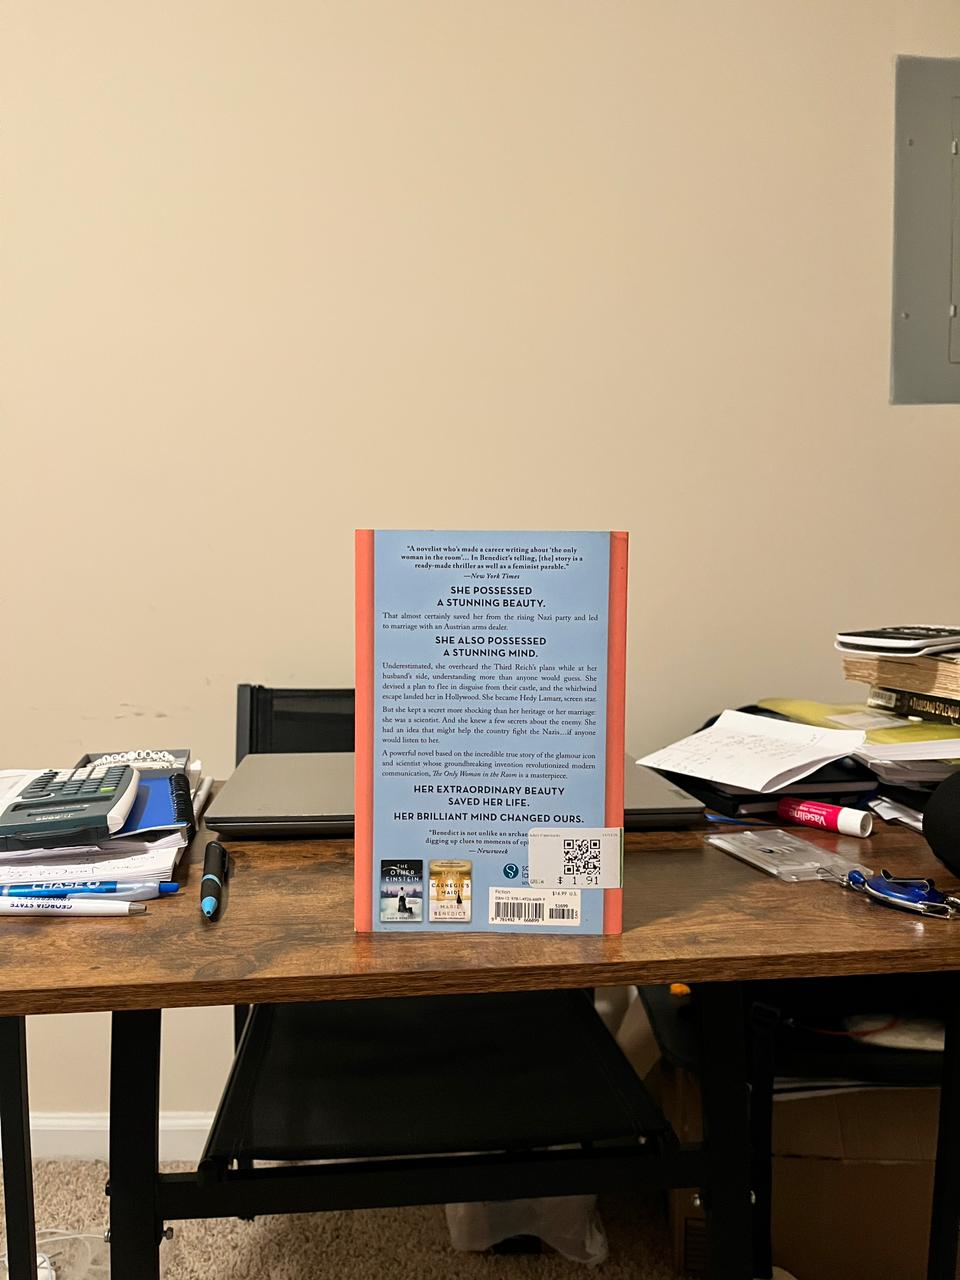
\includegraphics[width=\linewidth]{image_front.jpeg}
  \caption{Front}
\end{subfigure}
\begin{subfigure}{0.24\textwidth}
  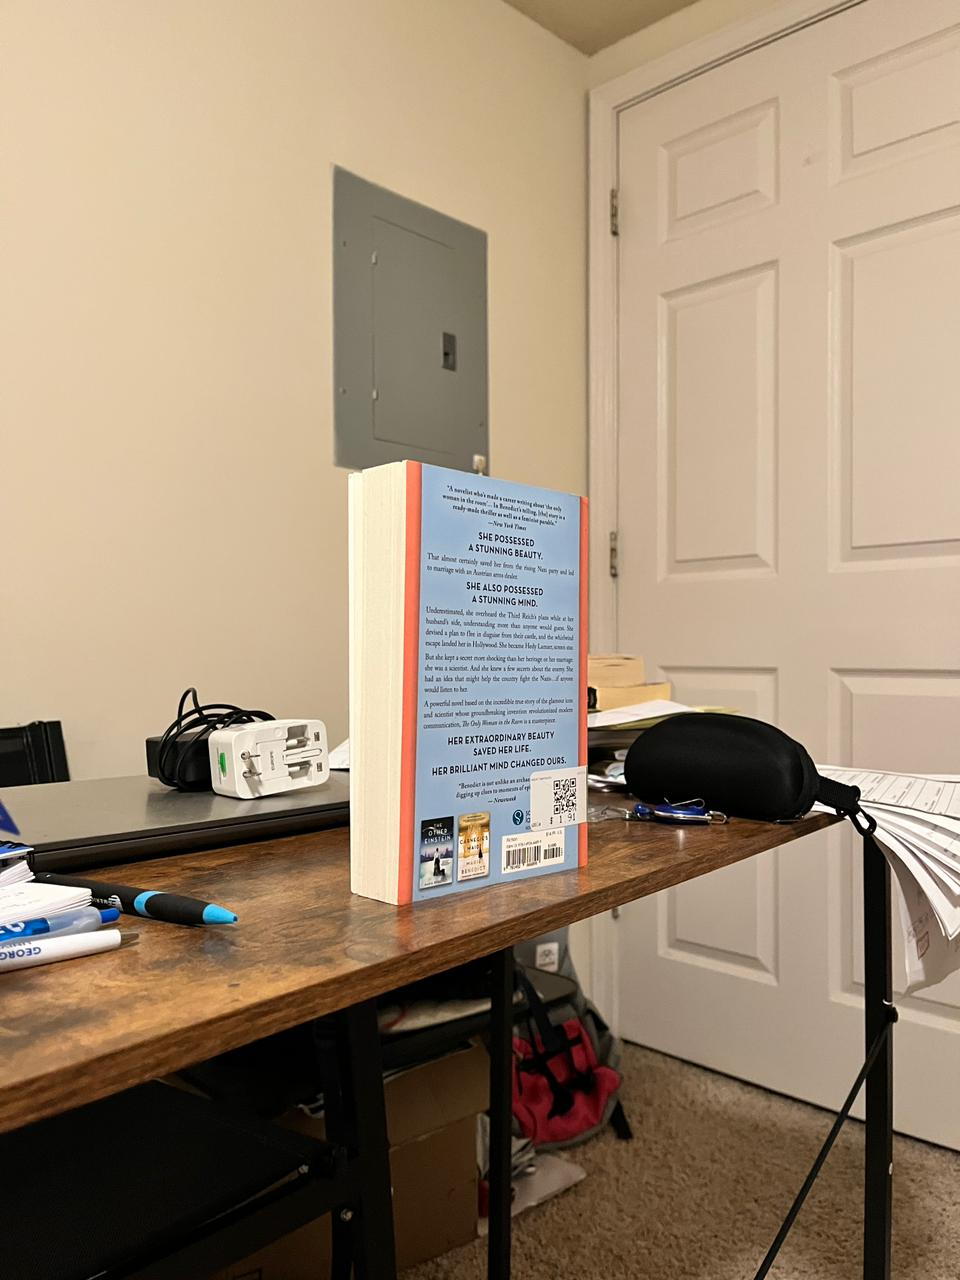
\includegraphics[width=\linewidth]{image_left.jpeg}
  \caption{Left}
\end{subfigure}
\begin{subfigure}{0.24\textwidth}
  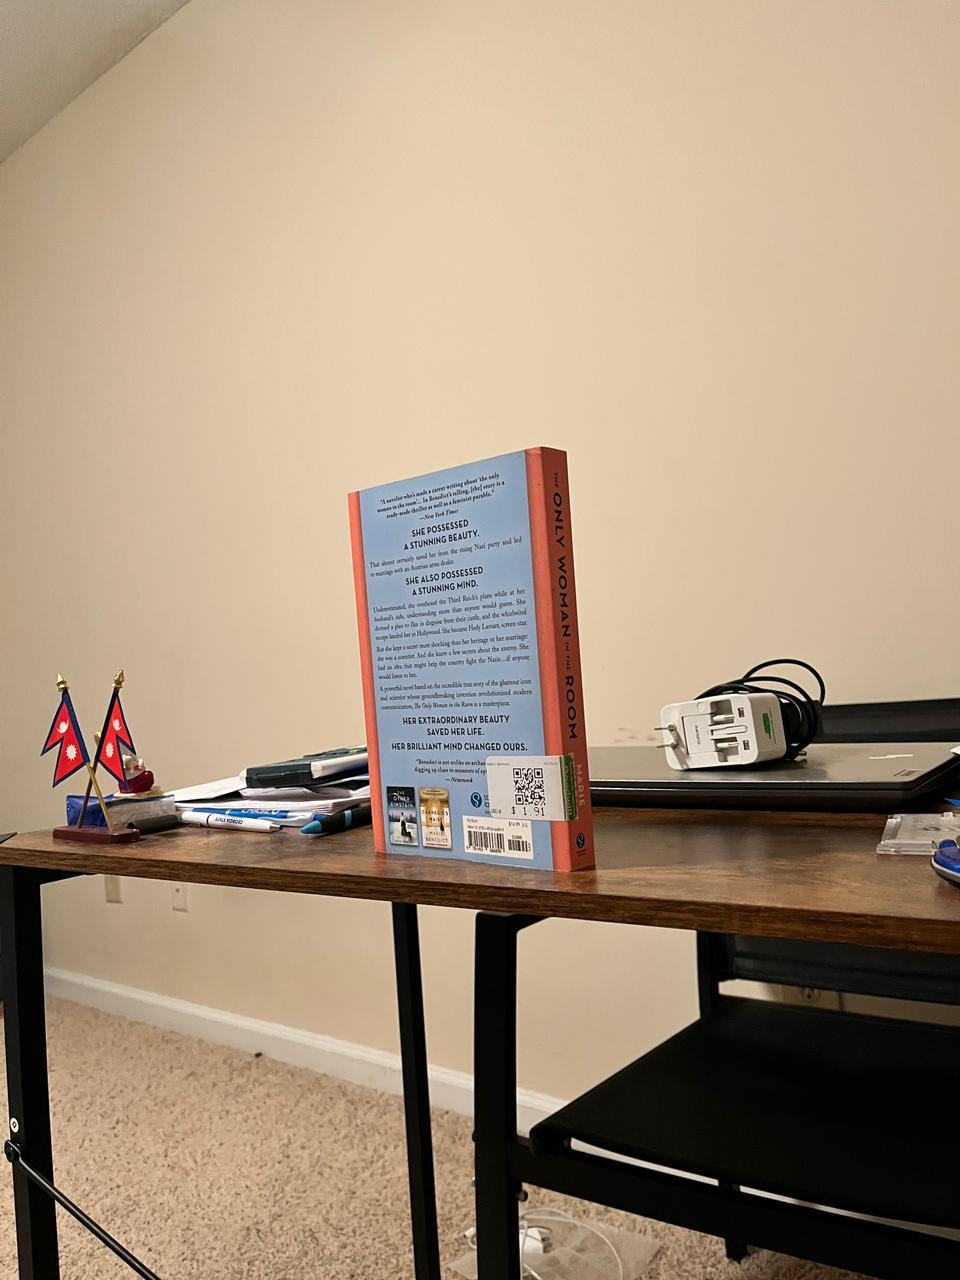
\includegraphics[width=\linewidth]{image_right.jpeg}
  \caption{Right}
\end{subfigure}
\begin{subfigure}{0.24\textwidth}
  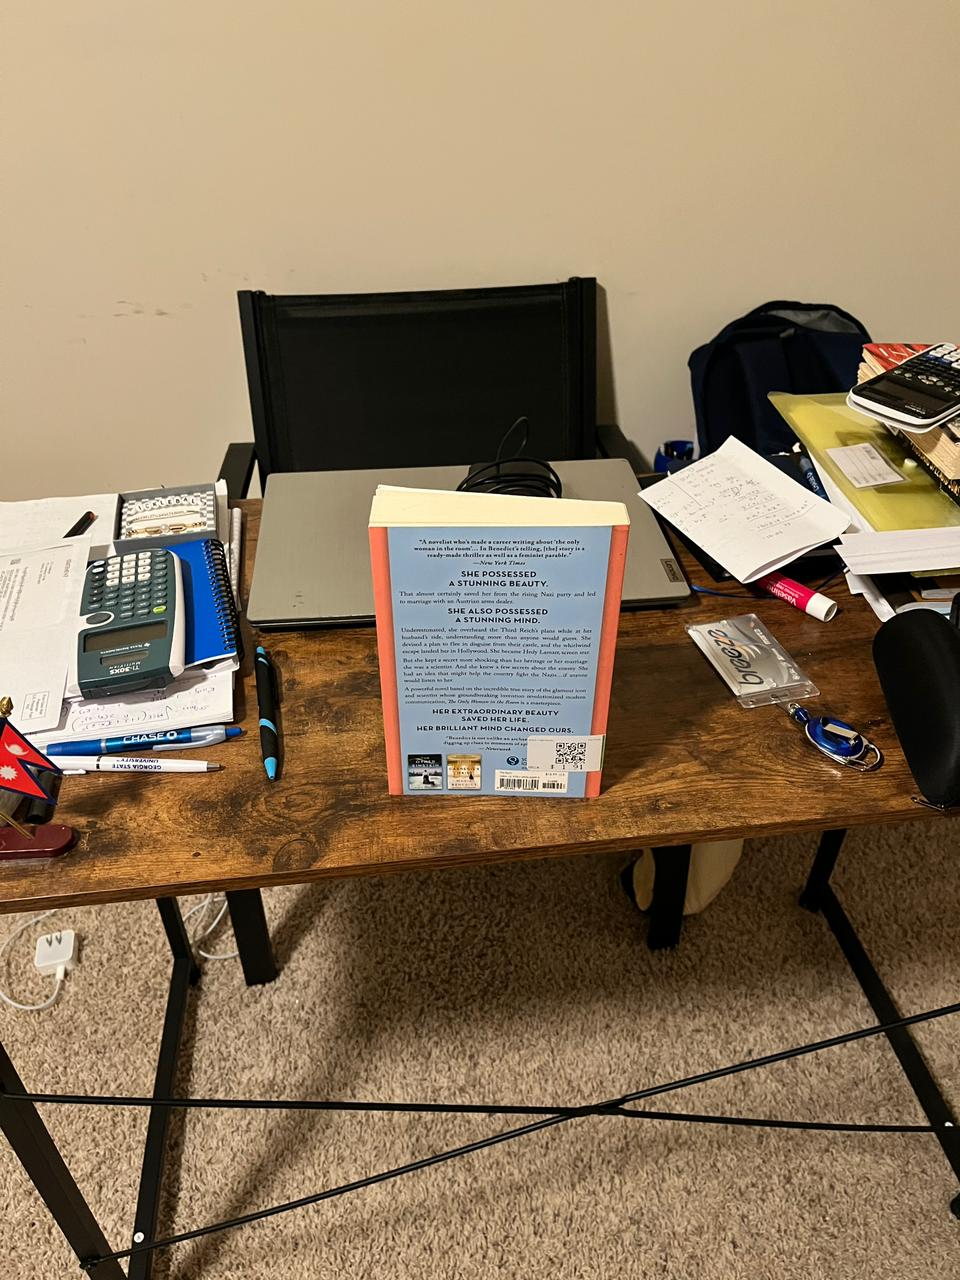
\includegraphics[width=\linewidth]{image_top.jpeg}
  \caption{Top}
\end{subfigure}
\caption{Four viewpoints of the book back cover used for SfM.}
\label{fig:sfm_views}
\end{figure}


% ------------------------------------------------------------------
\subsection{Mathematical Foundations}

\subsubsection{Homography for Planar Scenes}

A 3D world point $\mathbf{X} = (X, Y, Z, 1)^\top$ is projected to a pixel $\mathbf{x} = (u, v, 1)^\top$ via the pinhole camera model:
\begin{equation}
  \lambda\,\mathbf{x} = K\,[R \mid \mathbf{t}]\,\mathbf{X},
  \label{eq:pinhole}
\end{equation}
where $K$ is the $3\times3$ intrinsic matrix, $R$ is the $3\times3$ rotation matrix, $\mathbf{t}$ is the $3\times1$ translation vector, and $\lambda$ is a scalar.

If all object points lie on a plane (e.g.\ $Z=0$), writing $R = [\mathbf{r}_1\;\;\mathbf{r}_2\;\;\mathbf{r}_3]$:
\begin{equation}
  \lambda\,\mathbf{x} = K\,[\mathbf{r}_1\;\;\mathbf{r}_2\;\;\mathbf{r}_3\;\;\mathbf{t}]
  \begin{pmatrix}X\\Y\\0\\1\end{pmatrix}
  = K\,[\mathbf{r}_1\;\;\mathbf{r}_2\;\;\mathbf{t}]
  \begin{pmatrix}X\\Y\\1\end{pmatrix}.
\end{equation}

The $3\times3$ matrix mapping plane points to image points is the \textbf{homography}:
\begin{equation}
  H = K\,[\mathbf{r}_1\;\;\mathbf{r}_2\;\;\mathbf{t}].
  \label{eq:H_def}
\end{equation}

The inter-image homography between two views of the same plane is:
\begin{equation}
  H_{12} = K_2\left(R_{12} + \frac{\mathbf{t}_{12}\,\mathbf{n}^\top}{d}\right)K_1^{-1},
  \label{eq:H_inter}
\end{equation}
where $R_{12}$, $\mathbf{t}_{12}$ describe the relative pose, $\mathbf{n}$ is the plane normal, and $d$ is the distance to the plane.


\subsubsection{Direct Linear Transform (DLT)}

Given $N \geq 4$ point correspondences $(\mathbf{x}_i, \mathbf{x}'_i)$, the homography $H$ satisfying $\mathbf{x}_i \sim H\,\mathbf{x}'_i$ is found by solving:
\begin{equation}
  A\,\mathbf{h} = \mathbf{0},
\end{equation}
where $\mathbf{h} = \mathrm{vec}(H^\top)$ is the 9-vector of $H$ entries and each correspondence contributes two rows to $A$:
\[
  \begin{bmatrix}
    -u'_i & -v'_i & -1 & 0 & 0 & 0 & u_i u'_i & u_i v'_i & u_i\\
    0 & 0 & 0 & -u'_i & -v'_i & -1 & v_i u'_i & v_i v'_i & v_i
  \end{bmatrix}.
\]

\subsubsection{SVD Solution}

The solution $\ma\textbf{Point} & $x_0$ & $y_0$ & $x_{\text{pred}}$ & $y_{\text{pred}}$ & $x_{\text{act}}$ & $y_{\text{act}}$ & \textbf{Error (px)} \\
\midrule
1 & 500.0 & 221.0 & 501.4634 & 221.0399 & 501.0 & 221.0 & 0.4651 \\
2 & 423.0 & 199.0 & 424.3760 & 199.1626 & 424.0 & 199.0 & 0.4097 \\
3 & 472.0 & 220.0 & 473.4576 & 220.0781 & 474.0 & 220.0 & 0.5480 \\
4 & 499.0 & 195.0 & 500.4005 & 194.9882 & 500.0 & 195.0 & 0.4007 \\
5 & 472.0 & 192.0 & 473.4012 & 192.0552 & 473.0 & 192.0 & 0.4049 \\
6 & 410.0 & 170.0 & 411.2553 & 170.1575 & 411.0 & 170.0 & 0.3000 \\
7 & 511.0 & 138.0 & 512.1391 & 138.0040 & 512.0 & 138.0 & 0.1391 \\
8 & 679.0 & 325.0 & 679.7366 & 324.7141 & 680.0 & 325.0 & 0.3887 \\
\midrule
\multicolumn{7}{l}{\textbf{Mean Error}} & \textbf{0.3820} \\
\multicolumn{7}{l}{\textbf{Max Error}} & \textbf{0.5480} \\
\bottomrule
\end{tabular}
\end{table}

Figure~\ref{fig:tracking1} shows the validation image. Points in the first frame are marked, while predicted and actual positions in the second frame are overlaid for visual comparison.

\begin{figure}[H]
    \centering
    \includegraphics[width=0.95\textwidth]{cv_project_output/sample1_tracking_validation.jpg}
    \caption{Tracking validation visualization for \texttt{sample1.mp4}. Predicted positions and matched actual positions are nearly coincident, which agrees with the low error values in Table~\ref{tab:tracking1}.}
    \label{fig:tracking1}
\end{figure}

\subsection{Validation Results for sample2.mp4}
For \texttt{sample2.mp4}, frames 186 and 187 were selected, and points were chosen in a region of interest containing stronger water motion. The validation results are shown in Table~\ref{tab:tracking2}. The mean tracking error is 0.438999 pixels and the maximum error is 0.648365 pixels. The errors remain below one pixel, showing that the theoretical model still predicts motion accurately, although the sequence is more dynamic and locally irregular than the Earth sequence.

\begin{table}[H]
\centering
\caption{Tracking validation results for \texttt{sample2.mp4} using frames 186 and 187.}
\label{tab:tracking2}
\begin{tabular}{cccccccc}
\toprule
\textbf{Point} & $x_0$ & $y_0$ & $x_{\text{pred}}$ & $y_{\text{pred}}$ & $x_{\text{act}}$ & $y_{\text{act}}$ & \textbf{Error (px)} \\
\midrule
1 & 550.0 & 149.0 & 546.6020 & 150.1842 & 547.0 & 150.0 & 0.4385 \\
2 & 440.0 & 269.0 & 440.4835 & 268.9206 & 440.0 & 269.0 & 0.4900 \\
3 & 846.0 & 168.0 & 847.4028 & 168.3710 & 847.0 & 168.0 & 0.5476 \\
4 & 814.0 & 230.0 & 816.7655 & 230.1144 & 817.0 & 230.0 & 0.2610 \\
5 & 525.0 & 296.0 & 524.9806 & 295.9099 & 525.0 & 296.0 & 0.0921 \\
6 & 773.0 & 169.0 & 773.5116 & 169.3967 & 774.0 & 169.0 & 0.6292 \\
7 & 483.0 & 307.0 & 483.6336 & 306.8623 & 483.0 & 307.0 & 0.6484 \\
8 & 470.0 & 260.0 & 470.4051 & 260.0096 & 470.0 & 260.0 & 0.4052 \\
\midrule
\multicolumn{7}{l}{\textbf{Mean Error}} & \textbf{0.4390} \\
\multicolumn{7}{l}{\textbf{Max Error}} & \textbf{0.6484} \\
 & \textbf{Good Matches} & \textbf{RANSAC Inliers}\\
\midrule
front $\leftrightarrow$ left & 159 & 115\\
front $\leftrightarrow$ right & 226 & 165\\
front $\leftrightarrow$ top & 111 & 68\\
\bottomrule
\end{tabular}
\caption{Feature matching results across view pairs.}
\label{tab:matches}
\end{table}

\begin{figure}[H]
\centering
\includegraphics[width=\textwidth]{sfm_feature_matches.jpg}
\caption{SIFT feature matches between the front (reference) view and each other view. Lines connect matched keypoints.}
\label{fig:matches}
\end{figure}


\subsection{Homography Estimation and Warp Alignment}

Homographies were computed from each view to the front view using RANSAC.

\begin{figure}[H]
\centering
\includegraphics[width=\textwidth]{sfm_homography_warp.jpg}
\caption{Each view warped into the reference (front) coordinate frame using its estimated homography. The book region aligns correctly across all warps.}
\label{fig:warps}
\end{figure}


\subsection{Boundary Reconstruction}

The book boundary was detected in the reference view using the minimum-area bounding rectangle of all SIFT inlier points (which cluster on the book surface). This boundary was then projected to the other views via the inverse homographies.

\begin{figure}[H]
\centering
\includegraphics[width=\textwidth]{sfm_reconstructed_boundary.png}
\caption{Reconstructed book boundary across all four views. The red quadrilateral tightly wraps the book, confirming the homography estimation.}
\label{fig:boundary}
\end{figure}


\subsection{Camera Pose Recovery}

The homographies were decomposed to recover camera rotation $R$ and translation $\mathbf{t}$ for each view (Eqs.~\eqref{eq:r1}--\eqref{eq:t_recover}). Camera centres were computed using Eq.~\eqref{eq:cam_centre}.

\begin{figure}[H]
\centering
\includegraphics[width=0.7\textwidth]{sfm_camera_positions.png}
\caption{Estimated camera positions (triangles) and the object plane (cyan rectangle). The four cameras are positioned consistently with the front/left/right/top arrangement.}
\label{fig:cameras}
\end{figure}


% ======================================================================
%  CONCLUSION
% ======================================================================
\section{Conclusion}

This project demonstrated:

\begin{enumerate}
  \item \textbf{Dense optical flow} computation and visualisation using the Farneb\"{a}ck method, with quantitative evidence of motion patterns in two distinct videos.
  \item \textbf{Motion tracking} based on the brightness constancy assumption and the Lucas--Kanade formulation, validated with sub-pixel accuracy using exhaustive template matching.
  \item \textbf{Bilinear interpolation} for subpixel intensity estimation, derived from first principles and implemented in the tracker.
  \item \textbf{Structure from Motion} for a planar object using four viewpoints, including homography estimation via DLT/RANSAC, camera pose recovery, and boundary reconstruction.
\end{enumerate}

All mathematical derivations were provided, and the experimental results validate the theoretical framework.


% ======================================================================
%  REFERENCES
% ======================================================================
\section*{References}

\begin{enumerate}
  \item B.~D. Lucas and T.~Kanade, ``An Iterative Image Registration Technique with an Application to Stereo Vision,'' \emph{IJCAI}, 1981.
  \item B.~K.~P. Horn and B.~G. Schunck, ``Determining Optical Flow,'' \emph{Artificial Intelligence}, vol.~17, pp.~185--203, 1981.
  \item G.~Farneb\"{a}ck, ``Two-Frame Motion Estimation Based on Polynomial Expansion,'' \emph{SCIA}, 2003.
  \item R.~Szeliski, \emph{Computer Vision: Algorithms and Applications}, 2nd ed., Springer, 2022.
  \item R.~Hartley and A.~Zisserman, \emph{Multiple View Geometry in Computer Vision}, 2nd ed., Cambridge University Press, 2004.
  \item OpenCV Documentation, \url{https://docs.opencv.org/}.
\end{enumerate}

\end{document}
